\documentclass[svgnames,
               hyperref={colorlinks,citecolor=DeepPink4,linkcolor=FireBrick,urlcolor=Maroon},
               usepdftitle=false]  % see \hypersetup{} below
               {beamer}

\mode<presentation>{
  \usetheme{Madrid}
  \usecolortheme{seagull}
  \setbeamercovered{transparent}
  \setbeamerfont{frametitle}{size=\large}
}

\setbeamercolor*{block title}{bg=red!10}
\setbeamercolor*{block body}{bg=red!5}

%\usepackage[svgnames]{xcolor}
\usepackage{hyperref}
\hypersetup{
    pdftitle = {Making ice sheet models scale properly},
    pdfauthor = {Ed Bueler},
    pdfsubject = {},
    pdfkeywords = {}
}

\usepackage[english]{babel}
\usepackage[latin1]{inputenc}
\usepackage{times}
\usepackage[T1]{fontenc}
% Or whatever. Note that the encoding and the font should match. If T1
% does not look nice, try deleting the line with the fontenc.

\usepackage{empheq,bm}
\usepackage{xspace}
\usepackage{fancyvrb}

\usepackage{tikz}
\usetikzlibrary{shapes,arrows.meta,decorations.markings,decorations.pathreplacing,fadings,positioning}

\usepackage[kw]{pseudo}
\pseudoset{left-margin=15mm,topsep=5mm,idfont=\texttt,st-left=,st-right=}


% If you wish to uncover everything in a step-wise fashion, uncomment
% the following command:
%\beamerdefaultoverlayspecification{<+->}

\newcommand{\ba}{\mathbf{a}}
\newcommand{\bb}{\mathbf{b}}
\newcommand{\bc}{\mathbf{c}}
\newcommand{\bbf}{\mathbf{f}}
\newcommand{\bg}{\mathbf{g}}
\newcommand{\bn}{\mathbf{n}}
\newcommand{\bq}{\mathbf{q}}
\newcommand{\br}{\mathbf{r}}
\newcommand{\bx}{\mathbf{x}}
\newcommand{\by}{\mathbf{y}}
\newcommand{\bv}{\mathbf{v}}
\newcommand{\bu}{\mathbf{u}}
\newcommand{\bw}{\mathbf{w}}

\newcommand{\bF}{\mathbf{F}}
\newcommand{\bG}{\mathbf{G}}
\newcommand{\bQ}{\mathbf{Q}}

\newcommand{\grad}{\nabla}
\newcommand{\Div}{\nabla\cdot}

\newcommand{\argmin}{\operatorname{argmin}}

\newcommand{\CC}{\mathbb{C}}
\newcommand{\EE}{\mathbb{E}}
\newcommand{\RR}{\mathbb{R}}

\newcommand{\ddt}[1]{\ensuremath{\frac{\partial #1}{\partial t}}}
\newcommand{\ddx}[1]{\ensuremath{\frac{\partial #1}{\partial x}}}
\newcommand{\Matlab}{\textsc{Matlab}\xspace}
\newcommand{\Octave}{\textsc{Octave}\xspace}
\newcommand{\eps}{\epsilon}

\newcommand{\ip}[2]{\left<#1,#2\right>}

\newcommand{\xiphalf}{{x_{i+\frac{1}{2}}}}
\newcommand{\ximhalf}{{x_{i-\frac{1}{2}}}}
\newcommand{\Fiphalf}{{F_{i+\frac{1}{2}}}}
\newcommand{\Fimhalf}{{F_{i-\frac{1}{2}}}}
\newcommand{\Fiphalfn}{{F^n_{i+\frac{1}{2}}}}
\newcommand{\Fimhalfn}{{F^n_{i-\frac{1}{2}}}}

\newcommand{\trefcolumn}[1]{\begin{bmatrix} \phantom{x} \\ #1 \\ \phantom{x} \end{bmatrix}}
\newcommand{\trefmatrixtwo}[2]{\left[\begin{array}{c|c|c} & & \\ #1 & \dots & #2 \\ & & \end{array}\right]}
\newcommand{\trefmatrixthree}[3]{\left[\begin{array}{c|c|c|c} & & & \\ #1 & #2 & \dots & #3 \\ & & & \end{array}\right]}
\newcommand{\trefmatrixgroups}[4]{\left[\begin{array}{c|c|c|c|c|c} & & & & & \\ #1 & \dots & #2 & #3 & \dots & #4 \\ & & & & & \end{array}\right]}

\newcommand{\blocktwo}[4]{\left[\begin{array}{c|c} #1 & #2 \\ \hline #3 & #4 \end{array}\right]}

\newcommand{\bqed}{{\color{blue}\qed}}
\newcommand{\ds}{\displaystyle}

\newcommand\mynum[1]{{\renewcommand{\insertenumlabel}{#1}%
      \usebeamertemplate{enumerate item} \,}}


\title[Making ice sheet models scale properly]{Making ice sheet models \\ scale properly}

%\subtitle{\emph{x}}

\author{Ed Bueler}

\institute[UAF]{University of Alaska Fairbanks}

\date[]{February 2023}

%\titlegraphic{\begin{picture}(0,0)
%    \put(0,180){\makebox(0,0)[rt]{\includegraphics[width=4cm]{figs/software.png}}}
%  \end{picture}
%}

\titlegraphic{\hfill 
\includegraphics[width=0.2\textwidth]{images/uafbw.png}}

%% to start section counter at 0 see
%% https://tex.stackexchange.com/questions/170222/change-the-numbering-in-beamers-table-of-content


\begin{document}
\beamertemplatenavigationsymbolsempty

\begin{frame}
  \maketitle
\end{frame}


\begin{frame}{Outline}
  \tableofcontents[hideallsubsections]
\end{frame}


\section{what is an ice sheet model?}

\begin{frame}{what is an ice sheet?}

\begin{itemize}
\item before numerical models \dots \emph{what} are we modeling?
\item \emph{def.} an \alert{ice sheet} is a large glacier with small thickness$/$width ratio
\item<5> it is \emph{not} sea ice
\end{itemize}

\bigskip
\begin{minipage}[t][40cm][t]{\textwidth}
\begin{center}
\includegraphics<1>[height=0.64\textheight]{images/ant-pittard2021.png}
\only<1>{\par {\scriptsize Antarctic ice sheet (Pittard et al 2021)}}
\only<2>{\vspace{15mm}}
\includegraphics<2>[width=\textwidth]{images/ant-schoofhewitt2013.png}
\only<2>{\vspace{10mm}}
\only<2>{\par {\scriptsize note vertical exageration and rough bed (Schoof \& Hewitt 2013)}}
\includegraphics<3>[height=0.64\textheight]{images/alps-seguinot2018.png}
\only<3>{\par {\scriptsize modeled Alpine ice sheet near last glacial maximum (Seguinot et al 2018)}}
\includegraphics<4>[height=0.64\textheight]{images/british-clark2022.png}
\only<4>{\par {\scriptsize modeled British-Irish ice sheet near last glacial maximum (Clark et al 2022)}}
\includegraphics<5>[height=0.70\textheight]{images/not-sea-ice.png}
\end{center}
\end{minipage}
\end{frame}


\begin{frame}{what is an ice sheet model?}

\begin{columns}
\begin{column}{0.63\textwidth}
\begin{itemize}
\item ice is modeled as a non-Newtonian viscous fluid at large scale
    \begin{itemize}
    \item[$\circ$] more on that later \dots
    \end{itemize}
\item ice sheets evolve their geometry and velocity \emph{in contact with climate}
    \begin{itemize}
    \item[$\circ$] snowfall
    \item[$\circ$] surface melt
    \item[$\circ$] subglacial melt
    \item[$\circ$] melt and calving of parts which float in ocean (\emph{ice shelves})
    \end{itemize}
\end{itemize}
\end{column}
\begin{column}{0.4\textwidth}
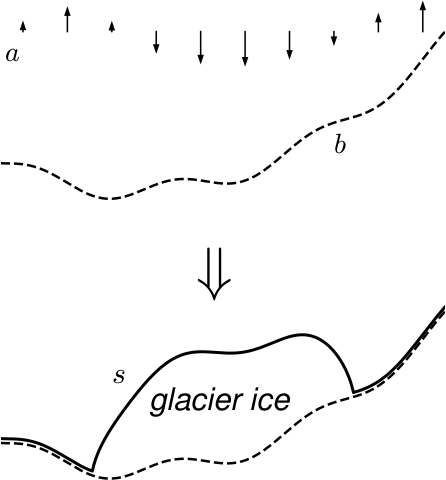
\includegraphics[width=\textwidth]{images/coverfig.png}
\end{column}
\end{columns}
\end{frame}


\begin{frame}{what is an ice sheet model?}

\begin{columns}
\begin{column}{0.63\textwidth}
\begin{itemize}
\item for purposes of clarity and analysis, let us simplify
\item inputs into an ice sheet model:
\item outputs from an ice sheet model:
\end{itemize}
\end{column}
\begin{column}{0.4\textwidth}
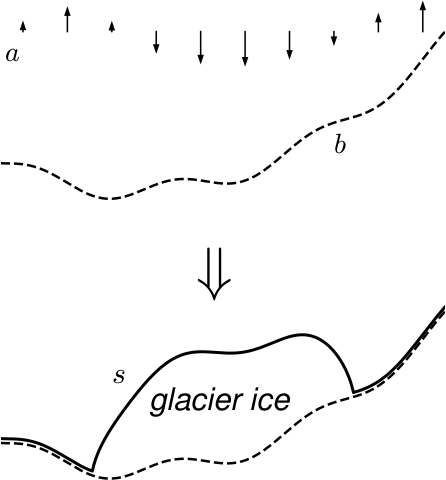
\includegraphics[width=\textwidth]{images/coverfig.png}
\end{column}
\end{columns}
\end{frame}


\begin{frame}{z}

\begin{itemize}
\item x
\item y
\end{itemize}
\end{frame}



\section{a simplified performance analysis}

\section{more on numerical stability}

\section{}

\begin{frame}{\alert{summary}}

\begin{itemize}
\item x
\item y
\end{itemize}
\end{frame}

\newcommand{\oo}[1]{\displaystyle O\left(#1\right)}

\begin{frame}{complexity table}

%\setlength{\tabcolsep}{5pt}
%\renewcommand{\arraystretch}{1.5}

\begin{tabular}{llll}
\emph{time-stepping} & \emph{dynamics} & \emph{flops per model year} & \emph{[pessimistic stability]} \\ \hline
explicit & SIA    & $\oo{\frac{D\, L^2}{\Delta x^4}} = \oo{\frac{D\, m^2}{L^2}}$ \\
explicit & Stokes & $\oo{\frac{U L^{2+2\alpha}}{\Delta x^{3+2\alpha}}} = \oo{\frac{U m^{1.5+\alpha}}{L}}$ & $\oo{\frac{D\, L^{2+2\alpha}}{\Delta x^{4+2\alpha}}} = \oo{\frac{D\,m^{2+\alpha}}{L^2}}$ \\
implicit & SIA    & $\oo{\frac{q\, L^{2+2\beta}}{\Delta x^{2+2\beta}}} = \oo{q\, m^{1+\beta}}$ \\
implicit & Stokes & $\oo{\frac{q\, L^{2+2\gamma}}{\Delta x^{2+2\gamma}}} = \oo{q\, m^{1+\gamma}}$
\end{tabular}

\begin{itemize}
\item Asymptotic estimates of algorithmic scaling, measured by floating point operations per model year, for map-plane (2D) time-stepping numerical ice sheet simulations, in the high resolution limit where $\Delta x\to 0$ and $m\to\infty$
\end{itemize}
\end{frame}


\begin{frame}{references}

\begin{itemize}
\footnotesize
\item E.~Hazan, A.~Agarwal, \& S.~Kale (2007).  \href{https://link.springer.com/content/pdf/10.1007/s10994-007-5016-8.pdf}{\emph{Logarithmic regret algorithms for online convex optimization.}} Machine Learning, 69(2), 169-192
    \begin{itemize}
    \scriptsize
    \item[$-$] $O(\log j)$ regret bounds for positive definite Hessians, and for Newton algorithms
    \end{itemize}
\item D.~P.~Kingma \& J.~Ba (2014). \href{https://arxiv.org/abs/1412.6980}{\emph{Adam: A method for stochastic optimization}}, preprint arXiv:1412.6980.
    \begin{itemize}
    \scriptsize
    \item[$-$] claims $O(\sqrt{j})$ regret bound
    \end{itemize}
\item M.~Zinkevich (2003). \href{https://www.aaai.org/Papers/ICML/2003/ICML03-120.pdf}{\emph{Online convex programming and generalized infinitesimal gradient ascent}}, Proceedings of the 20th International Conference on Machine Learning, 928-936
    \begin{itemize}
    \scriptsize
    \item[$-$] introduced regret
    \item[$-$] $O(\sqrt{j})$ regret bound of OGD
    \end{itemize}
\end{itemize}
\end{frame}




\end{document}
